


\section{Auswertung}
\label{sec:auswertung}

In diesem Kapitel werden die aufgenommenen Messwerte ausgewertet.

\subsection{Vermessung des Elektromagneten}
Es ist aufgrund des Versuchsaufbaus nicht möglich die magnetische Flussdichte $B$ zwischen den 
beiden Polschuhen des Elektromagneten zu bestimmen während die Cadmiumdampflampe eingeführt ist.
Daher muss das Magnetfeld vorher mittels einer Hallsonde in abhängigkeit vom Spulenstrom ausgemessen
werden. Wenn die Cadmiumdampflampe dann eingeführt ist muss nurnoch der passende Spulenstrom 
eingestellt werden. In \autoref{tab:magnetfeld} sind die Messdaten für die abfallende Seite der
Hysteresekurve dargestellt.
\begin{table}
    \centering
      \caption{In der Tabelle sind die Messdaten für den Spulenstrom $I$ und die resultierende Flussdichte $B$ dargestellt.}
      \label{tab:magnetfeld}
      \sisetup{table-format=1.2}
      \begin{tabular}{S[table-format=3.2] S S [table-format=3.2]}
        \toprule
        {$I$/[$\si[]{A}$]} & {$B$/[$\si[]{mT}$]}\\
        \midrule
        {$$5.0$$} & {$$ 452.1$$}\\
        {$$4.8$$} & {$$	440.4$$}\\
        {$$4.6$$} & {$$	430.2$$}\\
        {$$4.4$$} & {$$	415.4$$}\\
        {$$4.2$$} & {$$	403.4$$}\\
        {$$4.0$$} & {$$	388.0$$}\\
        {$$3.8$$} & {$$	371.7$$}\\
        {$$3.6$$} & {$$	356.7$$}\\
        {$$3.4$$} & {$$	338.8$$}\\
        {$$3.2$$} & {$$	320.9$$}\\
        {$$3.0$$} & {$$	305.5$$}\\
        {$$2.8$$} & {$$	288.2$$}\\
        {$$2.6$$} & {$$	266.8$$}\\
        {$$2.4$$} & {$$	248.8$$}\\
        {$$2.2$$} & {$$	229.6$$}\\
        {$$2.0$$} & {$$	209.2$$}\\
        {$$1.6$$} & {$$	169.8$$}\\
        {$$1.2$$} & {$$	131.1$$}\\
        {$$0.8$$} & {$$	89.4$$}\\
        {$$0.4$$} & {$$	50.7$$}\\
        {$$0.0$$} & {$$	 9.9$$}\\
        
        \bottomrule
      \end{tabular}
    \end{table}

    Die Daten aus \autoref{tab:magnetfeld} wurden in \autoref{fig:magnetfeld} dargestellt. Zudem wurde 
    an die Daten ein Polynom dritten Grades angepasst die verwendeten Parameter lauten:
    \begin{center}
        $$a_3 = -0.00105 \pm 0.00008$$\\
        $$a_2 =  0.00359 \pm 0.00062$$\\
        $$a_1 =  0.09673 \pm 0.00135$$\\
        $$a_0 =  0.01059 \pm 0.00080$$
        
    \end{center}

    \begin{figure}
        \centering
        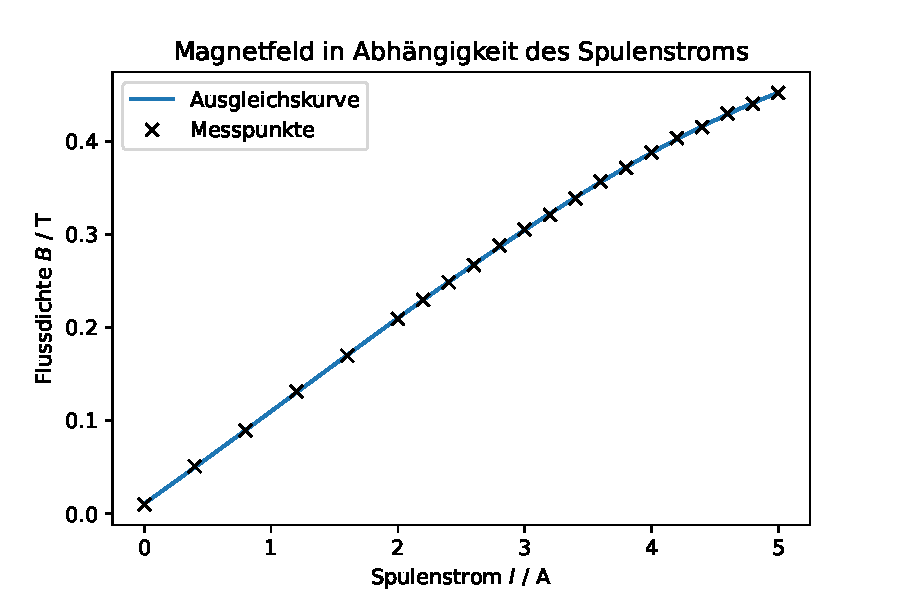
\includegraphics[width=1\textwidth]{content/grafiken/magnetfeld.pdf}
        \caption{Magnetische Flussdichte des verwendeten Elektromagneten in Abhängigkeit des Spulenstroms.}
        \label{fig:magnetfeld}
      \end{figure}